\documentclass{article}
\usepackage[utf8]{inputenc}
	\addtolength{\oddsidemargin}{-.875in}
		\addtolength{\textheight}{0.5in}
\usepackage{graphicx}
\usepackage[table,xcdraw]{xcolor}
\usepackage{amsmath}
\title{CON101 : Future Routing by Dr. S. C. Gupta}
\author{Anirudha Kulkarni}
\date{November 2020}
\usepackage{graphics}
\usepackage{hyperref}
\usepackage[export]{adjustbox}
\usepackage[table,xcdraw]{xcolor}
\usepackage[a4paper, total={6in, 8in}]{geometry}
\usepackage{multirow}
\usepackage{colortbl}
\usepackage{graphicx}
% \usepackage{multirow}
% \usepackage{colortbl}
\begin{document}

\maketitle
\section{Exercise 15}
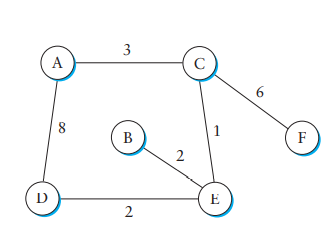
\includegraphics[center]{Assignment-4/ques.png}\\
For the network given in Figure, give global distance-vector tables like those
of Tables 4.5 and 4.8 when
(a) each node knows only the distances to its immediate neighbors.
(b) each node has reported the information it had in the preceding step to its
immediate neighbors.
(c) step (b) happens a second time.
\begin{table}[hbt]
\caption{When each node knows only the distances to its immediate neighbors.}
%\resizebox{\linewidth}{!}{%
\centering
\begin{tabular}{|c|c|c|c|c|c|c|} 
\hline
\multirow{2}{*}{InformationStored at Node} & \multicolumn{6}{c|}{Distance to Reach Node}                      \\ 
\cline{2-7}
                                           & A        & B        & C        & D        & E        & F         \\ 
\hline
A                                          & 0        & infinity & 3        & 8        & infinity & infinity  \\ 
\hline
B                                          & infinity & 0        & infinity & infinity & 2        & infinity  \\ 
\hline
C                                          & 3        & infinity & 0        & infinity & 1        & 6         \\ 
\hline
D                                          & 8        & infinity & infinity & 0        & 2        & infinity  \\ 
\hline
E                                          & infinity & 2        & 1        & 2        & 0        & infinity  \\ 
\hline
F                                          & infinity & infinity & 6        & infinity & infinity & 0         \\
\hline
\end{tabular}
%}
\arrayrulecolor{black}
\end{table}


\begin{table}[hbt!]
\caption{When each node has reported the information it had in the preceding step to its
immediate neighbors.}
\centering
\begin{tabular}{|c|c|c|c|c|c|c|} 
\hline
\multirow{2}{*}{Information Stored at Node} & \multicolumn{6}{c|}{Distance to Reach Node}        \\ 
\cline{2-7}
                                           & A        & B        & C & D        & E & F         \\ 
\hline
A                                          & 0        & infinity & 3 & 8        & 4 & 9         \\ 
\hline
B                                          & infinity & 0        & 3 & 4        & 2 & infinity  \\ 
\hline
C                                          & 3        & 3        & 0 & 3        & 1 & 6         \\ 
\hline
D                                          & 8        & 4        & 3 & 0        & 2 & infinity  \\ 
\hline
E                                          & 4        & 2        & 1 & 2        & 0 & 7         \\ 
\hline
F                                          & 9        & infinity & 6 & infinity & 7 & 0         \\
\hline
\end{tabular}

\arrayrulecolor{black}
\end{table}

% \usepackage{graphicx}
% \usepackage{multirow}
% \usepackage{colortbl}


\begin{table}[hbt!]
\caption{When step 2 happens a second time.}
\centering
\begin{tabular}{|c|c|c|c|c|c|c|} 
\hline
\multirow{2}{*}{Information Stored at Node} & \multicolumn{6}{c|}{Distance to Reach Node}  \\ 
\cline{2-7}
                                           & A & B & C & D & E & F                        \\ 
\hline
A                                          & 0 & 6 & 3 & 6 & 4 & 9                        \\ 
\hline
B                                          & 6 & 0 & 3 & 4 & 2 & 9                        \\ 
\hline
C                                          & 3 & 3 & 0 & 3 & 1 & 6                        \\ 
\hline
D                                          & 6 & 4 & 3 & 0 & 2 & 9                        \\ 
\hline
E                                          & 4 & 2 & 1 & 2 & 0 & 7                        \\ 
\hline
F                                          & 9 & 9 & 6 & 9 & 7 & 0                        \\
\hline
\end{tabular}

\arrayrulecolor{black}
\end{table}
\pagebreak{}

\pagebreak{}

\pagebreak{}

\section{Exercise 40}
\subsection{A possible arrangement of subnet masks}
Department A: 72 hosts, that is nearest power of 2 is 128. Hence addresses will be in the range 200.1.1.0 to 200.1.1.127. Hence subnet mask is 255.255.255.128\\
Department B: 35 hosts, that is nearest power of 2 is 64. Hence addresses will be in the range 200.1.1.128 to 200.1.1.191. Hence subnet mask is 255.255.255.192\\
Department C: 20 hosts, that is nearest power of 2 is 32. Hence addresses will be in the range 200.1.1.192 to 200.1.1.223. Hence subnet mask is 255.255.255.224\\
Department D: 18 hosts, that is nearest power of 2 is 32. Hence addresses will be in the range 200.1.1.224 to 200.1.1.255. Hence subnet mask is 255.255.255.224\\
\subsection{If department D grows to 34 hosts}
We can assign multiple subnets to a department to reduce vacant positions. Dividing A into 2 parts, we get 32 hosts and 40 hosts. Dividing subnets gives a subnet of 32 size and other with next power of 2 after 40, that is 64. So we are left with another 32 addresses which can be then used to allocate to Department D
\end{document}